\documentclass[conference]{IEEEtran}

% -
% KeySpark project paper.
%
% Compile:  latexmk -pdf main.tex      (or upload this folder to Overleaf,
%           which ships IEEEtran.cls and all packages used below).
%
% Items still to fill before submission are tagged  % TODO(data-freeze)
% (final dataset size + ML metrics) and  % TODO(figure)  (screenshots).
% Verify EVERY reference in references.bib against the real paper.
% -

\usepackage{cite}
\usepackage{amsmath,amssymb}
\usepackage{graphicx}
\usepackage{booktabs}
\usepackage{tikz}
\usetikzlibrary{positioning,arrows.meta,fit}
\usepackage{xcolor}
\usepackage[hidelinks]{hyperref}
\usepackage{url}

\begin{document}

\title{KeySpark: A Real-Time Stream-Processing Pipeline for\\
Keystroke and Mouse Behavioral Analytics}

\author{\IEEEauthorblockN{Murat Emirhan Aykut}
\IEEEauthorblockA{Bah\c{c}e\c{s}ehir University\\
Istanbul, T\"urkiye}}
% TODO(optional): add a contact / student email above if your professor wants one.

\maketitle

\begin{abstract}
Continuous human-computer interaction produces a high-rate, unbounded
stream of keyboard and mouse events that is a natural fit for modern
big-data stream-processing techniques. We present \emph{KeySpark}, an
end-to-end pipeline that captures input events on a host machine, ships
them through a distributed commit log (Apache Kafka), and analyzes them
with Apache Spark using a Lambda architecture: a Structured Streaming
\emph{speed layer} computes low-latency per-minute activity metrics over
event-time tumbling windows, while a periodic Spark \emph{batch layer}
computes order-dependent and session-level analytics (session
segmentation, a fatigue trend index, per-user baselines, and spatial
heatmaps). A leakage-free supervised model forecasts a user's next-minute
keystroke volume, and a web dashboard renders the results live. On a
single workstation the pipeline sustains a Structured Streaming
throughput of roughly $2.0\times10^{5}$ events/s at a mean micro-batch
latency of $275$\,ms, and a batch analytical throughput of roughly
$7.0\times10^{5}$ events/s, over an archive of
% TODO(data-freeze): final event count and collection span.
$\approx\!9.4\times10^{5}$ events collected over twelve days from one
user. The forecasting model improves root-mean-square error over a
persistence baseline by
% TODO(data-freeze): final RMSE/MAE/R2 from `ml evaluate`.
$\approx\!12\%$. We discuss the engineering trade-offs of the
speed/batch split, exactly-once delivery, and robustness to host
sleep/wake.
\end{abstract}

\begin{IEEEkeywords}
stream processing, Apache Spark, Apache Kafka, structured streaming,
Lambda architecture, behavioral analytics, keystroke dynamics.
\end{IEEEkeywords}

% ===========================================================================
\section{Introduction}
\label{sec:intro}
% - Problem Definition (rubric section 1) -

Knowledge work generates a continuous stream of low-level input events:
every key press, mouse movement, click, and scroll. Treated as data, this
is an \emph{unbounded, high-rate event stream}, exactly the regime that
big-data streaming systems are built for. Analyzing it in real time - to
surface productivity and fatigue signals while preserving privacy - is
both a useful application and a representative systems-engineering problem.

\textbf{Problem.} We address how to capture, transport, and analyze a
continuous stream of keyboard and mouse events such that (i) simple
per-minute activity metrics are available to a live dashboard at low
latency, (ii) richer, order-dependent and session-level analytics are
computed correctly, and (iii) the system tolerates real-world
disruptions such as the host machine sleeping and waking - all without
ever persisting the raw text the user types.

\textbf{Motivation.} Keystroke and mouse dynamics are an inexpensive,
content-free behavioral signal with established uses in authentication
and behavioral biometrics~\cite{monrose2000keystroke}. Beyond the
application, the data shape is a canonical big-data challenge: an
unbounded input that must be windowed on \emph{event time}, aggregated
incrementally, made fault-tolerant against producer/consumer rate
mismatch, and split between work that streaming can do cheaply and work
that fundamentally requires a bounded, fully ordered view.

\textbf{Objectives.} KeySpark is designed to:
\begin{itemize}
  \item ingest high-rate input events through a durable, replayable log
        that decouples capture from analysis (Apache Kafka);
  \item compute low-latency per-minute metrics with Spark Structured
        Streaming using event-time tumbling windows, watermarking, and
        an exactly-once columnar sink;
  \item compute order-dependent and session-scoped analytics in a Spark
        batch layer (the Lambda-architecture batch/serving side);
  \item forecast near-term user activity with a simple, leakage-free
        supervised model and report it honestly against naive baselines;
  \item serve all results to a live web dashboard; and
  \item remain robust to host sleep/wake, while persisting no raw
        keystroke content.
\end{itemize}

\textbf{Contributions.} (1) A complete, reproducible streaming-analytics
pipeline built from standard big-data components. (2) A concrete
justification for the Lambda speed/batch split, driven by metrics whose
correctness requires cross-batch ordering. (3) An honest empirical
evaluation reporting throughput, micro-batch latency, end-to-end latency,
and forecasting error against baselines.

% ===========================================================================
\section{Related Work}
\label{sec:related}

\textbf{Stream-processing foundations.} Apache Kafka introduced the
partitioned, replayable commit log as the substrate for decoupling event
producers from consumers~\cite{kreps2011kafka}; it is KeySpark's
ingestion bus. Apache Spark's resilient distributed
datasets~\cite{zaharia2012rdd} provide the fault-tolerant in-memory
engine, and its Structured Streaming API~\cite{armbrust2018structured}
models an unbounded stream as a continuously growing table so that the
same relational operators serve both batch and streaming - the model
KeySpark's speed layer uses directly. The Lambda
architecture~\cite{marz2015bigdata} pairs a low-latency speed layer with
a batch layer that acts as the source of truth; KeySpark is a
concrete, single-machine instantiation of this pattern, with the split
driven by metrics whose correctness requires cross-batch ordering
(Section~\ref{sec:batch}).

\textbf{Streaming systems over interaction data.} The closest
systems-level peers analyze continuous streams of user-interaction
events. Pal et al.~\cite{pal2023clickstream} build a Kafka-based
streaming pipeline over a high-velocity browser clickstream and forecast
the user's next clicks - closely analogous to KeySpark's
streaming-plus-forecast design, though over web clicks (via Apache Storm
and Markov chains) rather than keyboard and mouse events (via Spark
Structured Streaming and regression). Demirezen and
Navruz~\cite{demirezen2023lambda} apply the same Kafka-plus-Spark Lambda
stack in an unrelated domain, evidence of the pattern's generality.
Personal-productivity self-monitoring tools such as
TimeAware~\cite{kim2016timeaware} share the interaction-based,
per-time-bin measurement paradigm - its five-minute bins parallel
KeySpark's per-minute windows - but ingest periodically and track
application-usage time rather than streaming raw input events.
KeySpark's niche is thus a true streaming pipeline that computes live
metrics over raw keyboard and mouse events.

\textbf{Keystroke dynamics and state inference from typing.} Keystroke
dynamics - content-free timing features such as key hold and flight
times - are an established behavioral biometric for authentication and
identification~\cite{monrose2000keystroke,killourhy2009comparing,teh2013survey}.
KeySpark reuses the same content-free signals, but for productivity
and fatigue \emph{analytics} rather than identity, and never persists the
typed text. Typing patterns also carry affective and cognitive signal:
Epp et al.~\cite{epp2011identifying} showed that content-free keystroke
timing can classify a user's emotional state, and Acien et
al.~\cite{acien2022fatigue} recently detected mental fatigue from
keystroke dynamics with a deep network. KeySpark's fatigue index sits
in this lineage but is deliberately lightweight - an online
regression-slope trend over per-minute counts rather than an offline
deep model - and we treat it as a heuristic trend signal, not validated
fatigue detection. Mouse events are used only for a spatial-activity
visualization, not for state inference.

% ===========================================================================
\section{Dataset Description and Visualization}
\label{sec:dataset}
% - rubric section 3 --

\textbf{Source and collection.} The dataset is self-collected: a native
capture agent records the host's keyboard and mouse events during normal
use. Each event is emitted as a JSON record carrying the event
\texttt{type}, a coarse key identifier or pointer coordinates, the user
id, and an event timestamp \texttt{ts}.
% TODO(data-freeze): final number of events and the collection window.
At the time of writing the archive holds $\approx\!9.4\times10^{5}$
events spanning twelve days from a single user.

\textbf{Privacy by construction.} The agent stores a stable key
\emph{identifier} (the character for printable keys, a symbolic name for
special keys) for timing and counting only; \textbf{no raw typed text is
ever persisted}. Mouse-move events are throttled to roughly $50$/s to
bound volume; clicks and scrolls are never throttled.

\textbf{Format and schema.} Events are parsed into a typed schema
(\texttt{type, key, x, y, button, pressed, dx, dy, user, ts}) and stored
as columnar Parquet, the de-facto analytics format.

\textbf{Features / derived signals.} From the raw events the pipeline
derives, per one-minute window, four counts - keystrokes, words (space
presses), corrections (backspace/delete), and clicks - plus
session-level trend slopes and per-user means and standard deviations
(Section~\ref{sec:arch}).

\textbf{Pre-processing.} Parsing applies an explicit schema (avoiding
costly inference); a watermark bounds late/out-of-order events; mouse
moves are throttled at capture; and idle windows are handled with
divide-by-zero guards in derived ratios.
% TODO(figure): dataset visualization - e.g., histogram of keystrokes
% per window and/or the dashboard's per-minute time series.

% ===========================================================================
\section{Proposed Solution and System Architecture}
\label{sec:arch}
% - rubric section 4 (the core systems contribution) --

\begin{figure*}[t]
\centering
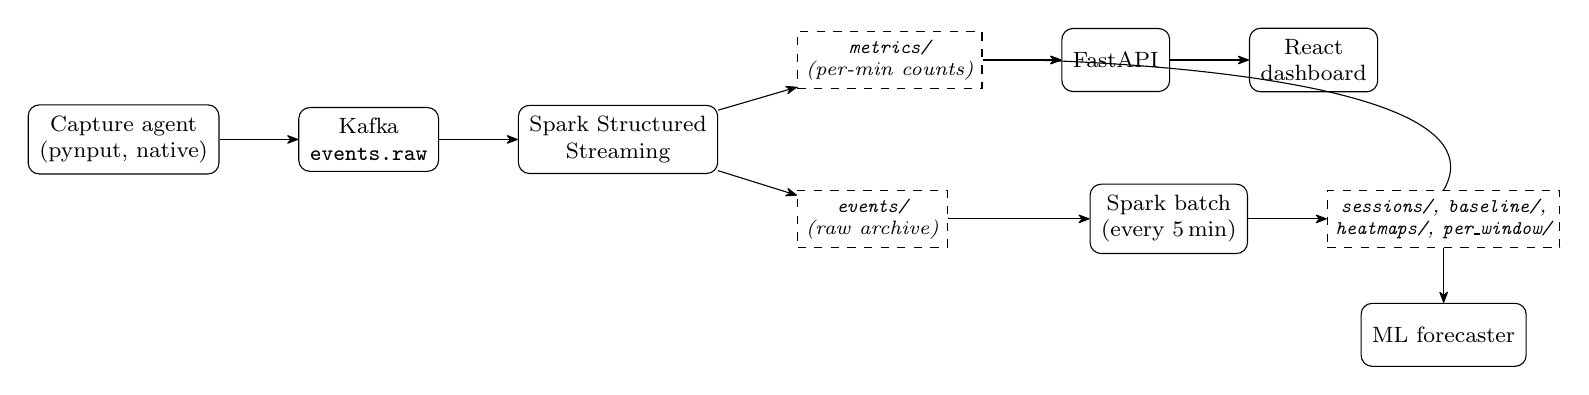
\begin{tikzpicture}[
  >={Stealth[round]},
  box/.style={draw, rounded corners, align=center, font=\footnotesize,
              minimum height=8mm, inner sep=4pt},
  store/.style={draw, dashed, align=center, font=\scriptsize\itshape,
                minimum height=7mm, inner sep=3pt},
  node distance=7mm and 10mm
]
  \node[box] (agent) {Capture agent\\(pynput, native)};
  \node[box, right=of agent] (kafka) {Kafka\\\texttt{events.raw}};
  \node[box, right=of kafka] (stream) {Spark Structured\\Streaming};
  \node[store, above right=2mm and 10mm of stream] (metrics) {\texttt{metrics/}\\(per-min counts)};
  \node[store, below right=2mm and 10mm of stream] (events) {\texttt{events/}\\(raw archive)};
  \node[box, right=18mm of events] (batch) {Spark batch\\(every 5\,min)};
  \node[store, right=of batch] (analytics) {\texttt{sessions/}, \texttt{baseline/},\\\texttt{heatmaps/}, \texttt{per\_window/}};
  \node[box, below=of analytics] (ml) {ML forecaster};
  \node[box, right=of metrics] (api) {FastAPI};
  \node[box, right=of api] (dash) {React\\dashboard};

  \draw[->] (agent) -- (kafka);
  \draw[->] (kafka) -- (stream);
  \draw[->] (stream) -- (metrics);
  \draw[->] (stream) -- (events);
  \draw[->] (events) -- (batch);
  \draw[->] (batch) -- (analytics);
  \draw[->] (analytics) -- (ml);
  \draw[->] (metrics) -- (api);
  \draw[->] (analytics.north) to[out=60,in=180] (api.west);
  \draw[->] (api) -- (dash);
\end{tikzpicture}
\caption{KeySpark data flow. The agent produces JSON events to Kafka;
Spark Structured Streaming writes per-minute metrics and a raw event
archive; a Spark batch job derives session, baseline, and heatmap
analytics plus the ML forecaster's training table; FastAPI serves the
Parquet outputs to the dashboard.}
\label{fig:arch}
\end{figure*}

Figure~\ref{fig:arch} shows the five stages: capture, ingestion, stream
processing, batch processing, and serving. We describe each in turn and
justify the key design decisions.

\subsection{Capture agent}
The agent runs as a native host process because the operating-system
input event tap is not reachable from inside a container. It emits one
JSON event per input action to either standard output (for verification)
or Kafka. It is resilient to host sleep/wake: on wake it re-establishes
the event listeners, and a watchdog detects a silently dead listener and
exits so a supervisor restarts a clean process.

\subsection{Ingestion: Kafka as a replayable log}
The agent does not call Spark directly; it appends each event to the
Kafka topic \texttt{events.raw}, keyed by user~\cite{kreps2011kafka}.
Kafka is a distributed, append-only, partitioned log: it (i) decouples
the producer from the consumer in both time and rate, (ii) persists
events so a consumer can be restarted or replayed without loss, and
(iii) presents the ``unbounded stream'' that Structured Streaming treats
as a growing input table. We run a single broker in KRaft mode, which
removes the former ZooKeeper dependency, in a container.

\subsection{Speed layer: Spark Structured Streaming}
\label{sec:streaming}
The streaming job consumes \texttt{events.raw}, casts each Kafka value to
a string, and parses it with an \emph{explicit} schema (avoiding the cost
and unpredictability of schema inference). It then runs two queries that
share one parsed stream:

\begin{itemize}
  \item \textbf{Query A (metrics).} Events are grouped into one-minute
        \emph{tumbling} windows per user and aggregated into four counts
        (keystrokes, words, corrections, clicks), written once per
        finalized window to \texttt{metrics/}.
  \item \textbf{Query B (archive).} The parsed events are written
        verbatim to \texttt{events/}, the durable, ordered record the
        batch layer consumes.
\end{itemize}

Four streaming concepts are central to correctness:

\textbf{Event time vs.\ processing time.} Windows are defined on the
event's own timestamp, not on when Spark happens to process it. A
``typing minute'' is one minute of real keyboard activity.

\textbf{Watermarking.} Because events can arrive late or out of order,
a watermark (here $5$\,s) tells Spark how long to wait before it
considers a window's result final and frees its state.

\textbf{Append output mode.} The Parquet file sink supports only append
mode, which emits each window's row exactly once. Append on a windowed
aggregation is only sound \emph{with} a watermark, since otherwise Spark
could never decide a window is complete.

\textbf{Checkpointing and exactly-once.} Each query checkpoints its Kafka
offsets (and Query~A its window state); combined with the Parquet sink's
atomic, log-based commits, output is end-to-end exactly-once and resumes
cleanly after a restart~\cite{armbrust2018structured}.

\subsection{Batch layer: order-dependent analytics}
\label{sec:batch}
Some signals cannot be computed correctly on a live stream. Session
boundaries and inter-keystroke timing depend on the \emph{previous}
event, and a \texttt{lag} window function does not see across streaming
micro-batches, so such a computation would silently miss every gap that
straddles a batch boundary. We therefore adopt the Lambda split: the
speed layer lands every event durably and emits the simple counts, and a
batch job over the bounded event archive is the source of truth for
order-dependent and session-level analytics. The batch job runs every
five minutes from an in-process scheduler in the API service. It reads
the full event archive via a file glob (so it processes every recorded
event, independent of the streaming sink's commit log) and computes:

\begin{itemize}
  \item \textbf{Sessions} via the gap-and-island pattern: ordering each
        user's events by event time, flagging a new session whenever the
        idle gap exceeds five minutes, and taking a running cumulative
        sum of those flags as a stable integer session id.
  \item \textbf{A fatigue trend index} per session. Using the SQL
        \texttt{regr\_slope} aggregate, we fit the per-minute keystroke
        and correction counts against the within-session minute index;
        the index combines a falling typing rate and a rising correction
        rate. A reliability flag suppresses the index for sessions with
        too few windows to fit a meaningful slope.
  \item \textbf{Per-user baselines} (mean and standard deviation of each
        per-minute metric), enabling z-score comparison of new activity.
  \item \textbf{Spatial heatmaps} per preset time range, by binning
        pointer coordinates into a fixed grid - spatial windowing
        analogous to time windowing.
\end{itemize}

\subsection{Forecasting model}
\label{sec:ml}
On top of the batch outputs we train a one-step-ahead regressor that
predicts a user's \emph{next} one-minute keystroke count from the last
three windows of the current session (lagged keystroke, word, correction,
and click counts) plus the minute index within the session and the
wall-clock hour. Using only past windows to predict a future value makes
the task leakage-free by construction. We use a random-forest
regressor~\cite{breiman2001random,pedregosa2011scikit} and evaluate it on
a chronological hold-out (train on the earliest windows, test on the most
recent), comparing against a \emph{persistence} baseline (next minute
equals the current minute) and a \emph{mean} baseline. Results are in
Section~\ref{sec:results}.

\subsection{Serving layer and deployment}
A small FastAPI service reads the Parquet outputs and serves them as JSON;
a React dashboard polls these endpoints and renders live metric cards, a
per-minute time series, the spatial heatmaps, and the session table. We
run Spark in \texttt{local[*]} mode because we process a single user's
stream and do not need a cluster; Kafka runs in a container; only the
capture agent must be native. Each long-running process is wrapped in a
restart loop, which together with Spark checkpointing and the Kafka log
gives the pipeline its sleep/wake resilience.

% ===========================================================================
\section{Results and Discussion}
\label{sec:results}
% - rubric section 5 --

\subsection{Throughput and latency}
We benchmark on the recorded archive on a single workstation
(\texttt{local[*]} Spark). Table~\ref{tab:perf} reports the batch
analytical throughput and the Structured Streaming throughput and
per-micro-batch latency, both measured from Spark's own progress metrics.
% TODO(data-freeze): re-run `python -m streamguard.benchmark batch` and
% `... streaming` on the final archive and update the numbers below.

\begin{table}[t]
\caption{Processing performance on the event archive (single machine).}
\label{tab:perf}
\centering
\begin{tabular}{lrr}
\toprule
Layer & Throughput & Latency \\
\midrule
Spark batch (full pipeline) & $\approx\!7.0\times10^{5}$ ev/s & - \\
Structured Streaming        & $\approx\!2.0\times10^{5}$ ev/s & $275$\,ms / batch \\
End-to-end (capture$\to$UI) & -                             & $\approx\!65$\,s \\
\bottomrule
\end{tabular}
\end{table}

The batch layer attains higher per-event throughput because it processes
the archive in a single pass with no per-micro-batch overhead or
watermark-state management; the streaming layer trades some throughput
for incremental, low-latency processing. The $\approx\!65$\,s end-to-end
latency is dominated \emph{by design} by the one-minute window plus the
watermark, not by engine speed: a per-minute metric cannot be finalized
until its minute has elapsed.

\subsection{Forecasting accuracy}
% TODO(data-freeze): paste the final numbers from `ml evaluate` into the
% table below (model vs.\ persistence vs.\ mean; RMSE, MAE, R2) and update
% the prose. Current draft values are from an interim run.
Table~\ref{tab:ml} reports root-mean-square error (RMSE), mean absolute
error (MAE), and $R^2$ on the chronological hold-out. The model beats both
naive baselines, reducing RMSE over persistence by $\approx\!12\%$ and
posting a positive $R^2$ where both baselines are negative. The dominant
features are the previous minute's keystroke count and the minute index
within the session, which matches intuition: near-term typing volume is
the best predictor of the next minute, modulated by where one is in a
session.

\begin{table}[t]
\caption{Next-minute keystroke forecast (chronological hold-out).}
\label{tab:ml}
\centering
\begin{tabular}{lrrr}
\toprule
Predictor & RMSE & MAE & $R^2$ \\
\midrule
Random forest (ours) & $77.1$ & $60.0$ & $+0.12$ \\ % TODO(data-freeze)
Persistence baseline & $88.1$ & $61.1$ & $-0.14$ \\ % TODO(data-freeze)
Mean baseline        & $82.8$ & $67.4$ & $-0.01$ \\ % TODO(data-freeze)
\bottomrule
\end{tabular}
\end{table}

\subsection{Demonstration}
The live system is demonstrated by typing and watching the per-minute
metrics, time series, and heatmaps update on the dashboard within the
window-plus-watermark latency, with the Spark UI's Structured Streaming
tab showing input and processing rates in real time.
% TODO(figure): dashboard screenshot and Spark UI streaming-tab screenshot.

\subsection{Limitations and future work}
The deployment is single-broker, single-user, and single-machine
(\texttt{local[*]}); a multi-user or clustered deployment would exercise
Kafka partitioning and Spark shuffle behavior more fully. The fatigue
index is a heuristic trend, not a clinically validated measure. The
end-to-end latency is bounded below by the one-minute window; a shorter
window would lower it at the cost of noisier per-minute labels. Host
sleep long enough to tear down Spark's local RPC forces a process restart,
so recovery is on the order of a Spark cold start rather than seconds.
Future work includes multi-user/clustered deployment, richer rhythm
features for the forecaster, and an anomaly-detection mode scoring live
windows against the per-user baseline.

% ===========================================================================
\section{Conclusion}
\label{sec:conclusion}
KeySpark shows that a continuous stream of input events can be
captured, transported, and analyzed end to end with standard big-data
components. A Lambda architecture cleanly separates low-latency per-minute
metrics (Structured Streaming) from order-dependent, session-level
analytics (Spark batch), and a simple leakage-free model forecasts
near-term activity above naive baselines. On a single machine the pipeline
sustains hundreds of thousands of events per second while preserving user
privacy by never storing typed content.

% ===========================================================================
\bibliographystyle{IEEEtran}
\bibliography{references}

\end{document}
